% System model -- short version for a paper (same method as system_model.tex, which has every detail).
% Formulation-4 RL: 2026-11-22_formulation_4/baseline_RL/code.  Compile: pdflatex system_model_concise.tex
\documentclass[border=4pt]{standalone}
\usepackage{lmodern}
\usepackage[T1]{fontenc}
\usepackage{amsmath,amssymb}
\usepackage{graphicx}
\usepackage{tikz}
\usetikzlibrary{arrows.meta,shapes.geometric,fit,backgrounds,calc}
\begin{document}
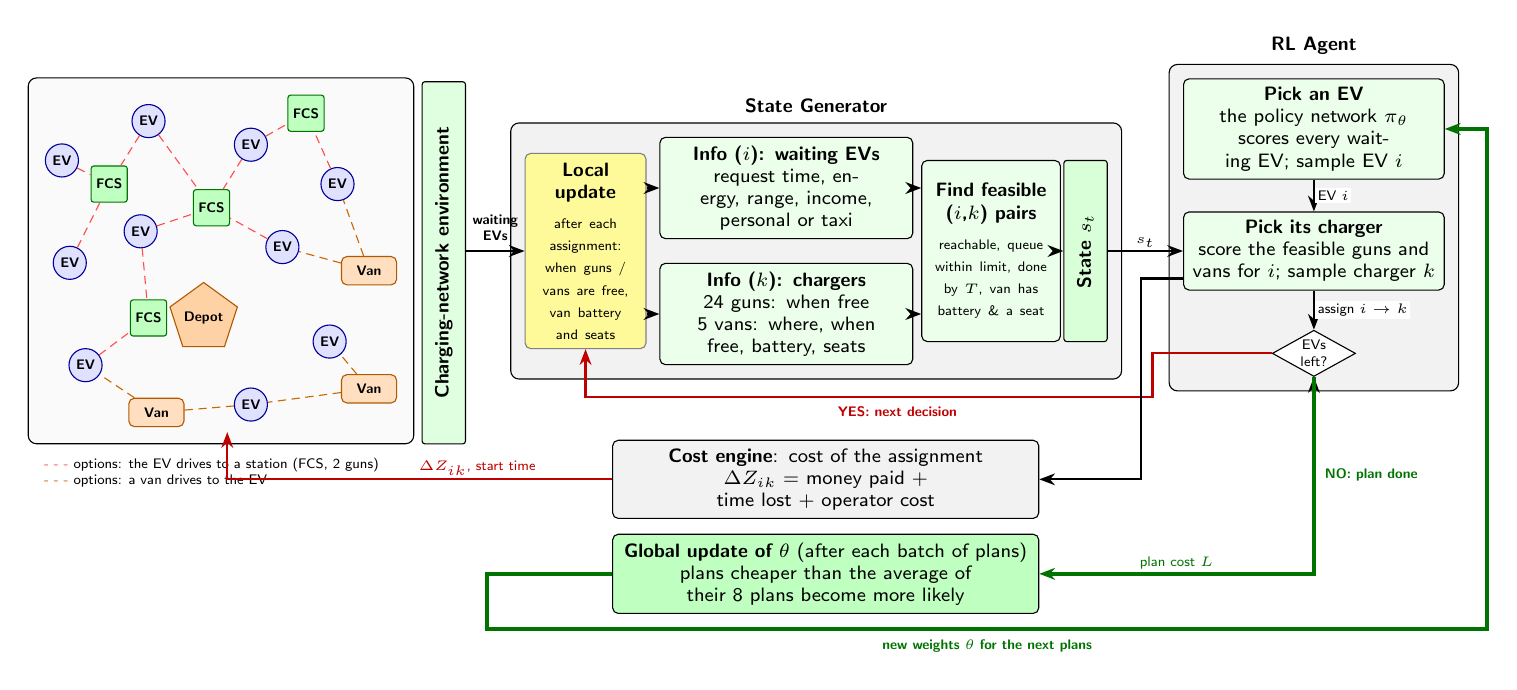
\begin{tikzpicture}[
  font=\sffamily\scriptsize, >={Stealth[length=2mm]},
  ev/.style={circle, draw=blue!60!black, fill=blue!12, inner sep=1pt, minimum size=4.2mm, font=\sffamily\tiny\bfseries},
  fcs/.style={rectangle, rounded corners=1pt, draw=green!45!black, fill=green!25, minimum size=4.6mm, inner sep=0pt, font=\sffamily\tiny\bfseries},
  van/.style={rectangle, rounded corners=2pt, draw=orange!70!black, fill=orange!25, minimum width=7mm, minimum height=3.6mm, inner sep=0pt, font=\sffamily\tiny\bfseries},
  opt/.style={red!70, densely dashed, thin},
  box/.style={draw, rounded corners=2pt, align=center, fill=white, inner sep=3pt},
  card/.style={box, fill=green!8},
  flow/.style={->, thick},
  back/.style={->, thick, red!75!black},
  upd/.style={->, very thick, green!45!black},
  tag/.style={font=\sffamily\tiny, fill=white, inner sep=1pt},
]
% ===================================================== environment (left), x 0..4.6
\node[regular polygon, regular polygon sides=5, draw=orange!70!black, fill=orange!35, minimum size=9mm, inner sep=0pt, font=\sffamily\tiny\bfseries] (dep) at (2.0,0.9) {Depot};
\foreach \n/\x/\y in {a/0.2/2.9, b/1.3/3.4, c/2.6/3.1, d/3.7/2.6, e/0.3/1.6, f/1.2/2.0, g/3.0/1.8, h/0.5/0.3, i/3.6/0.6, j/2.6/-0.2}
  \node[ev] (\n) at (\x,\y) {EV};
\node[fcs] (s1) at (0.8,2.6) {FCS};
\node[fcs] (s2) at (2.1,2.3) {FCS};
\node[fcs] (s3) at (3.3,3.5) {FCS};
\node[fcs] (s4) at (1.3,0.9) {FCS};
\node[van] (v1) at (4.1,1.5) {Van};
\node[van] (v2) at (4.1,0.0) {Van};
\node[van] (v3) at (1.4,-0.3) {Van};
\foreach \e/\s in {a/s1, b/s1, b/s2, c/s2, c/s3, d/s3, e/s1, f/s2, f/s4, g/s2, h/s4}
  \draw[opt] (\e) -- (\s);
\foreach \v/\e in {v1/d, v1/g, v2/i, v2/j, v3/h, v3/j}
  \draw[opt, orange!80!black] (\v) -- (\e);
\begin{scope}[on background layer]
  \node[draw, rounded corners=3pt, fill=gray!4, fit=(a)(b)(s3)(v1)(v2)(v3)(h), inner sep=6pt] (envbox) {};
\end{scope}
\node[draw, fill=green!12, rounded corners=1pt, minimum width=5.5mm, minimum height=4.6cm] (strip) at (5.05,1.6)
  {\rotatebox{90}{\textbf{Charging-network environment}}};
\node[font=\sffamily\tiny, anchor=north west, align=left] at (-0.15,-0.75)
  {\textcolor{red!70}{- - -} options: the EV drives to a station (FCS, 2 guns)\\
   \textcolor{orange!80!black}{- - -} options: a van drives to the EV};

% ===================================================== state generator, x 6..13.4
\node[draw=black!50, fill=yellow!40, rounded corners=2pt, align=center, text width=1.3cm, minimum height=2.3cm] (local) at (6.85,1.75)
  {\textbf{Local update}\\[3pt]\tiny after each assignment: when guns / vans are free, van battery and seats};
\node[card, text width=3.0cm] (infoi) at (9.4,2.55) {\textbf{Info ($i$): waiting EVs}\\ request time, energy, range, income, personal or taxi};
\node[card, text width=3.0cm] (infok) at (9.4,0.95) {\textbf{Info ($k$): chargers}\\ 24 guns: when free\\ 5 vans: where, when free, battery, seats};
\node[card, text width=1.55cm, minimum height=2.3cm] (feas) at (12.0,1.75)
  {\textbf{Find feasible ($i$,$k$) pairs}\\[3pt]\tiny reachable, queue within limit, done by $T$, van has battery \& a seat};
\node[draw, fill=green!15, minimum width=5.5mm, minimum height=2.3cm, rounded corners=1pt] (st) at (13.2,1.75)
  {\rotatebox{90}{\textbf{State $s_t$}}};
\begin{scope}[on background layer]
  \node[draw, fill=gray!10, rounded corners=3pt, fit=(local)(infoi)(infok)(feas)(st), inner sep=5pt,
        label={[font=\sffamily\scriptsize\bfseries]above:State Generator}] (sg) {};
\end{scope}

% ===================================================== RL agent, x 14.3..17.9
\node[card, text width=3.1cm] (pick1) at (16.1,3.3) {\textbf{Pick an EV}\\ the policy network $\pi_\theta$ scores every waiting EV; sample EV $i$};
\node[card, text width=3.1cm] (pick2) at (16.1,1.75) {\textbf{Pick its charger}\\ score the feasible guns and vans for $i$; sample charger $k$};
\node[diamond, draw, fill=white, aspect=1.8, inner sep=0.6pt, align=center, font=\sffamily\tiny] (left) at (16.1,0.45) {EVs\\left?};
\begin{scope}[on background layer]
  \node[draw, fill=gray!10, rounded corners=3pt, fit=(pick1)(pick2)(left), inner sep=5pt,
        label={[font=\sffamily\scriptsize\bfseries]above:RL Agent}] (ag) {};
\end{scope}

% ===================================================== bottom: cost engine, global update
\node[box, fill=gray!10, text width=5.2cm] (cost) at (9.9,-1.15)
  {\textbf{Cost engine}: cost of the assignment\\ $\Delta Z_{ik}$ = money paid + time lost + operator cost};
\node[box, fill=green!25, text width=5.2cm] (glob) at (9.9,-2.35)
  {\textbf{Global update of $\theta$} (after each batch of plans)\\ plans cheaper than the average of their 8 plans become more likely};

% ===================================================== arrows
\draw[flow] (strip.east|-local.west) -- node[above, align=center, font=\sffamily\tiny\bfseries]{waiting\\EVs} (local.west);
\draw[flow] (local.east|-infoi.west) -- (infoi.west);
\draw[flow] (local.east|-infok.west) -- (infok.west);
\draw[flow] (infoi.east) -- (feas.west|-infoi.east);
\draw[flow] (infok.east) -- (feas.west|-infok.east);
\draw[flow] (feas) -- (st);
\draw[flow] (st.east) -- node[above, tag]{$s_t$} (pick2.west|-st.east) ;
\draw[flow] (pick1) -- node[right, tag]{EV $i$} (pick2);
\draw[flow] (pick2) -- node[right, tag]{assign $i\to k$} (left);
% YES: next decision -> local update
\draw[back] (left.west) -- (14.05,0.45) -- (14.05,-0.1) -- node[below, font=\sffamily\tiny\bfseries, pos=0.45]{YES: next decision} (6.85,-0.1) -- (local.south);
% assignment -> cost engine -> environment
\draw[flow] (left.south) ++(0,0) coordinate (ls);
\draw[flow] ($(pick2.west)+(0,-0.35)$) -- (13.9,1.4) -- (13.9,-1.15) -- (cost.east);
\draw[back] (cost.west) -- node[above, tag, pos=0.35]{$\Delta Z_{ik}$, start time} (2.3,-1.15) -- (2.3,-0.55);
% NO: plan complete -> global update -> new theta to agent
\draw[upd] (left.south) -- node[right, font=\sffamily\tiny\bfseries]{NO: plan done} (16.1,-2.35) -- node[above, tag]{plan cost $L$} (glob.east);
\draw[upd] (glob.west) -- (5.6,-2.35) -- (5.6,-3.05) -- node[below, font=\sffamily\tiny\bfseries, pos=0.5]{new weights $\theta$ for the next plans} (18.3,-3.05) -- (18.3,3.3) -- (pick1.east);
\end{tikzpicture}
\end{document}
